\subsection{} On fait osciller un chariot contenant deux briques relié à deux ressorts. Si on enlève une des deux briques, la fréquence de l’oscillation sera-t-elle augmentée, diminuée ou inchangée ? Justifiez votre réponse.
\begin{center}
    \centering
    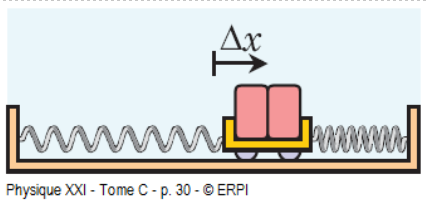
\includegraphics[width=0.45 \linewidth]{Figures/chariot_deux_briques.png}
\end{center}

\noindent\textbf{Réponse :} \hrulefill \\[2.5ex]
\rule{\linewidth}{0.4pt} \\[2.5ex]
\rule{\linewidth}{0.4pt}
\vfill